\documentclass{article}

\usepackage{color}
\usepackage{listings}
\usepackage{fullpage}
\usepackage{graphicx}

\definecolor{gray_ulisses}{gray}{0.55}
\definecolor{castanho_ulisses}{rgb}{0.71,0.33,0.14}
\definecolor{preto_ulisses}{rgb}{0.41,0.20,0.04}
\definecolor{green_ulises}{rgb}{0.2,0.75,0}

\lstdefinelanguage{HaskellUlisses}
{
	basicstyle=\ttfamily\scriptsize,
	%backgroundcolor=\color{yellow},
	%frameshape={RYRYNYYYY}{yny}{yny}{RYRYNYYYY}, %contornos... muito nice...
	sensitive=true,
	morecomment=[l][\color{gray_ulisses}\scriptsize]{--},
	morecomment=[s][\color{gray_ulisses}\scriptsize]{\{-}{-\}},
	morestring=[b]",
	stringstyle=\color{red},
	showstringspaces=false,
	numbers=none,
	firstnumber=\thelstnumber,
	numberstyle=\tiny,
	numberblanklines=true,
	showspaces=false,
	showtabs=false,
	xleftmargin=15pt,
	xrightmargin=-20pt,
	emph=
	{[1]
		FilePath,IOError,abs,acos,acosh,all,and,any,appendFile,approxRational,asTypeOf,asin,
		asinh,atan,atan2,atanh,basicIORun,break,catch,ceiling,chr,compare,concat,concatMap,
		const,cos,cosh,curry,cycle,decodeFloat,denominator,digitToInt,div,divMod,drop,
		dropWhile,either,elem,encodeFloat,enumFrom,enumFromThen,enumFromThenTo,enumFromTo,
		error,even,exp,exponent,fail,filter,flip,floatDigits,floatRadix,floatRange,floor,
		fmap,foldl,foldl1,foldr,foldr1,fromDouble,fromEnum,fromInt,fromInteger,fromIntegral,
		fromRational,fst,gcd,getChar,getContents,getLine,head,id,inRange,index,init,intToDigit,
		interact,ioError,isAlpha,isAlphaNum,isAscii,isControl,isDenormalized,isDigit,isHexDigit,
		isIEEE,isInfinite,isLower,isNaN,isNegativeZero,isOctDigit,isPrint,isSpace,isUpper,iterate,
		last,lcm,length,lex,lexDigits,lexLitChar,lines,log,logBase,lookup,map,mapM,mapM_,max,
		maxBound,maximum,maybe,min,minBound,minimum,mod,negate,not,notElem,null,numerator,odd,
		or,ord,otherwise,pi,pred,primExitWith,print,product,properFraction,putChar,putStr,putStrLn,quot,
		quotRem,range,rangeSize,read,readDec,readFile,readFloat,readHex,readIO,readInt,readList,readLitChar,
		readLn,readOct,readParen,readSigned,reads,readsPrec,realToFrac,recip,rem,repeat,replicate,return,
		reverse,round,scaleFloat,scanl,scanl1,scanr,scanr1,seq,sequence,sequence_,show,showChar,showInt,
		showList,showLitChar,showParen,showSigned,showString,shows,showsPrec,significand,signum,sin,
		sinh,snd,span,splitAt,sqrt,subtract,succ,sum,tail,take,takeWhile,tan,tanh,threadToIOResult,toEnum,
		toInt,toInteger,toLower,toRational,toUpper,truncate,uncurry,undefined,unlines,until,unwords,unzip,
		unzip3,userError,words,writeFile,zip,zip3,zipWith,zipWith3,Impl,Equiv,Prop,Neg,Cnj,Dsj
	},
	emphstyle={[1]\color{blue}},
	emph=
	{[2]
		Bool,Char,Double,Either,Float,IO,Integer,Int,Maybe,Ordering,Rational,Ratio,ReadS,ShowS,String,NoTriangle,Equilateral,Rectangular,Isosceles,Other,Shape
	},
	emphstyle={[2]\color{castanho_ulisses}},
	emph=
	{[3]
		case,class,data,deriving,do,else,if,import,in,infixl,infixr,instance,let,
		module,of,primitive,then,type,where
	},
	emphstyle={[3]\color{preto_ulisses}\textbf},
	emph=
	{[4]
		quot,rem,div,mod,elem,notElem,seq
	},
	emphstyle={[4]\color{castanho_ulisses}\textbf},
	emph=
	{[5]
		EQ,False,GT,Just,LT,Left,Nothing,Right,True,Show,Eq,Ord,Num
	},
	emphstyle={[5]\color{preto_ulisses}\textbf}
}

\lstnewenvironment{code}
{\lstset{language=HaskellUlisses}}
{\smallskip}


\begin{document}
\setlength{\parindent}{0cm}
\title{Software Testing Assignment 4}
\author{Cindy Berghuizen, Omar Pakker , Chiel Peter, Maria Gouseti}
\date{\today}
\maketitle
\section*{1: Book Exercise}

\subsection*{Chapter 4}
\begin{itemize}
\item Prove of Theorem 4.38.2 on page 135.  Don't understand the last steps of both parts.
\end{itemize}
\subsection*{Chapter 5}
Lot's of definition page after page so it gets difficult to get through the chapter because you need to remember all the definitions and symbols to know exactly what you are reading. There are much exercises so there wasn't really enough time to get far enough to really get into trouble. Further more I (Cindy) have more trouble with the number theory related to the relations than with the definitions of the relations itself (when it starts about prime numbers or modulo...)
\section*{2: Random data generator}

\begin{code}
genSetMax = 100
genSetMaxEntries = 10

genSet :: IO (Set Int)
genSet =  do
   n  <- getRandomInt genSetMaxEntries
   ns <- genSet' genSetMax n
   return ns

genSet' :: (Eq a, Num a) => Int -> a -> IO (Set Int)
genSet' _ 0 = return (Set [])
genSet' d c = do
         n <- getRandomInt d
         ns <- genSet' d (c-1)
         return (insertSet n ns)

\end{code}
Time spent: 10 minutes

\section*{Set intersectiom, union, difference}

\subsection*{Haskell Program}
\begin{code}
intersectSet :: (Ord a) => Set a -> Set a -> Set a 
intersectSet (Set [])     set2  =  (Set [])
intersectSet (Set (x:xs)) set2  | inSet x set2 = insertSet x (intersectSet (Set xs) set2)
                                | otherwise = (intersectSet (Set xs) set2)

-- Pre: no duplicates, it is sorted
-- Post: no duplicates, it is sorted 
differenceSet :: (Ord a) => Set a -> Set a -> Set a
differenceSet (Set [])     set2  =  (Set [])
differenceSet (Set (x:xs)) set2  | inSet x set2 = (differenceSet (Set xs) set2)
                                 | otherwise = insertSet x (differenceSet (Set xs) set2)                             

--Union is already implemented in SetOrd.hs
\end{code}

Union was already implemented in SetOrd.hs\\

\subsection*{Intersection Test}
The property of an Intersection set is the following: \\
\emph{
Property: A set I is an intersection of sets A and B if the elements of I are in A and B.
$ A \cap B := \left\{ x: x \in A \land x \in B\right\} $ \\}

We test by calling function automatedI. This function generates two random sets and calculates the intersection of those sets. To see if the intersection set indeed is the intersection of A and B we check if it is an subset of A and a subset of B in the function testIntersect. This function returns True is that is the case. The function generateIntersectionTest is used to test multiple cases, this function returns True if all testcases return True.

\begin{code}
-- A set I is an intersection of A and B if I is an subset of A and B 
testIntersect :: (Ord a) => Set a -> Set a -> Set a -> Bool
testIntersect a b i = subSet i a && subSet i b

automatedI :: IO Bool
automatedI = do
    a <- genSet
    b <- genSet
    return $ testIntersect a b (intersectSet a b)

automatedI' :: Int -> IO [Bool]
automatedI' 0 = return []
automatedI' c = do
     d <- automatedI
     ds <- automatedI'(c-1)
     return (d:ds)
     
generateIntersectionTest :: Int -> IO String
generateIntersectionTest c = do
    ps <- automatedI' c
    return ("All Checks Valid: " ++ (show (all (\x -> x) ps)))
\end{code}

\subsection*{Difference Test}
The property from a Difference set is the following:\\
 \emph{
An set D is the difference of A and B if its element are in A and it has no elements in common with B. Also written as:
$ A \setminus B := \left\{ x: x \in A \land x \not \in B\right\} $ }\\

The testing is done by inserting two random sets in the function automatedD and calculating the difference of those two sets. Next, we will check that the differenceset is indeed a subset of set A and that the difference set has no elements in common with set B. If this is the case the differenceSet is correct and the function automatedD will return True. 

For testing multiple sets we can make use of the function generateDifferenceTest. This will result in True if all the testcases return true in atomatedD.

\begin{code}
-- Property: An set D is the difference of A and B if it is an subset
--  of A and has no elements in common with B                        
testDifference :: (Ord a) => Set a -> Set a -> Set a -> Bool
testDifference a b d = subSet d a && noElement d b

noElement :: (Ord a) => Set a -> Set a -> Bool
noElement (Set[]) _ = True
noElement (Set(x:xs)) set | inSet x set = False
                          | otherwise = noElement (Set xs) set
                          
automatedD :: IO Bool
automatedD = do
    a <- genSet
    b <- genSet
    return $ testDifference a b (differenceSet a b)

automatedD' :: Int -> IO [Bool]
automatedD' 0 = return []
automatedD' c = do
     d <- automatedD
     ds <- automatedD'(c-1)
     return (d:ds)
     
generateDifferenceTest :: Int -> IO String
generateDifferenceTest c = do
    ps <- automatedD' c
    return ("All Checks Valid: " ++ (show (all (\x -> x) ps)))
\end{code}

\subsection*{Union Test}
The property to test of a union set is the following: \\ \emph{
Every element in either of the sets should be an element of the union set.
$ A \cup B := \left\{ x: x \in A \lor x \in B\right\} $ }\\

To test this we use the function isElementOf. isElementOf gets a set A, a set B and the presumable union set of A and B. It then tests if every element in the unionset is an element in set A or in set B. If this is the case the function will return True. To check multiple cases testUnion can be used. This returns the list of all the results of the test cases.

\begin{code}
--PROPERTY : Every element in either of the sets should be an element of the union
testUnion :: Int -> IO [Bool]
testUnion 0 = return []
testUnion a = do 	n <- testUnion1
			ns <- testUnion (a-1)			
			return(n : ns)

testUnion1 :: IO Bool
testUnion1 = do 	n <- randomIntSet
			m <- randomIntSet
			return(isElementOf n m (unionSet n m)) 

isElementOf :: (Ord a) => Set a -> Set a -> Set a -> Bool
isElementOf (Set a) (Set b) (Set c) = all (\x -> elem x c) (a++b)
\end{code}

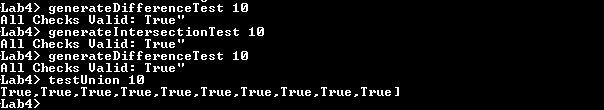
\includegraphics{knipsel}

\newpage
Time spent: 75 minutes

\section*{Transitive Closure}
\begin{code}
trClos :: (Ord a) => Rel a -> Rel a
trClos x = trClos2 x []

-- If the closure n+1 is a subset of n than all closures are found
-- because no new elements were found
trClos2 :: (Ord a) => Rel a -> Rel a -> Rel a
trClos2  = fix (\ f x y ->
           if subSet (list2set x) (list2set y) then (nub x)
           else f ((x @@ x)++x) x) 
\end{code}

Time spent: 1.5 hours

\section*{Testing Closure}
For testing the closure we use the following property: \\
\emph{If the relations (x,y) and (y,z) exist in a transitiveclosure, then the relation (x,z) should exist in the transitive closure set. This can also be written as: \\
$\left\{ (x,y) , (y,z) \in R^+ \rightarrow(x,z) \in R^+ \right\}$}\\

The function testTrClos tests if a relation has the transitive closure property. This could easily be tested by checking if for a relation {\em R} it holds that
 {\em R} is equal to the transitive closure of  {\em R}. However since we are testing our function trClos we can not assume trClos gives the transitive closure. Therefore we tested the property above. The function testTrClos receives the relationship twice, it recurses over the first input and the second remains the relation itself. It checks if for every element in  {\em R} the above property holds. Then the test is randomized by first making a randomrelation function and then test if the TrClos holds for the random relations. Bigger input then 10 is also inspected however for visual purposes 10 was chosen in the graphic below.

\begin{code}
testTrClos :: (Ord a) => Rel a -> Rel a -> Bool
testTrClos [] _ = True
testTrClos (x:xs) z = (all (\y -> elem y z) ([x] @@ z)) && (testTrClos xs z)

--RANDOM TESTING
randomTestsTrClos :: Int -> IO [Bool]
randomTestsTrClos 0 = return []
randomTestsTrClos a = do 	n <- randomTestTrClos
				m <- randomTestsTrClos (a-1)
				return (n:m)

randomTestTrClos :: IO Bool
randomTestTrClos = do 	n <- randomRelation maxSize
			return( testTrClos (trClos n) (trClos n)) 

randomRelation :: (Eq a, Num a) => a -> IO [(Int,Int)]
randomRelation 0 = return []
randomRelation a = do 	n <- getRandomInt range
			m <- getRandomInt range
			l <- randomRelation (a-1)
			return((n,m):l) 

\end{code}

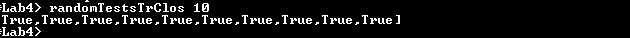
\includegraphics{knipsel2}

Time spent: 2 hours

\end{document}